\section*{Math 202A - HW7 - Dan Davison - \texttt{ddavison@berkeley.edu}}

\begin{mdframed}
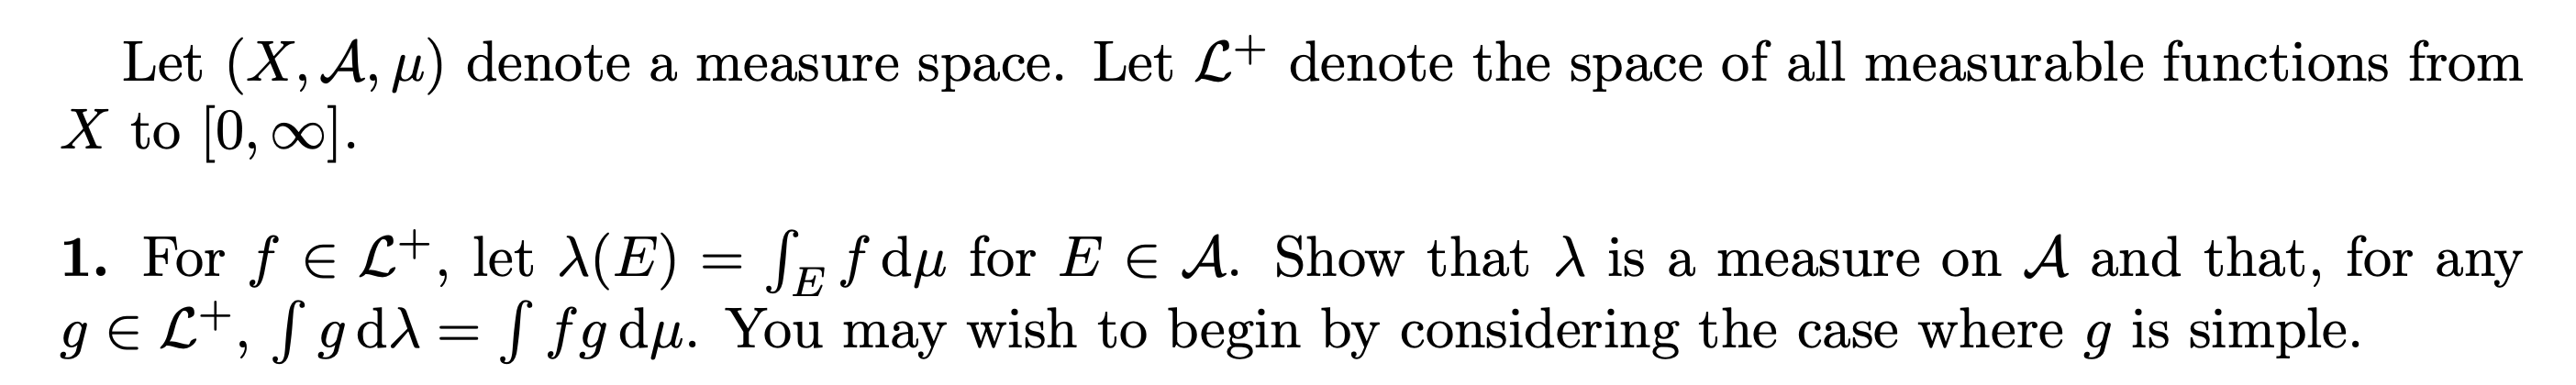
\includegraphics[width=400pt]{img/analysis--berkeley-202a-hw07-9f9b.png}
\end{mdframed}

\begin{lemma}[Finite additivity of integral]\label{lemma-finite-additivity-of-integral}
  Let $E_1 \ldots E_n \in \mc A$ be pairwise disjoint and let $f \in \mc L^+$. Then
  \begin{align*}
    \int_{\bigcup_{i=1}^n E_i} f = \sum_{i=1}^n \int_{E_i}f.
  \end{align*}
\end{lemma}

\begin{proof}
  We have
  \begin{align*}
    \int_{E_1 \cup E_2} f
    &= \int_{E_1 \cup E_2} (f\ind_{E_1} + f\ind_{E_2}) \\
    &= \int_{E_1 \cup E_2} f\ind_{E_1} + \int_{E_1 \cup E_2} f\ind_{E_2} ~~~~~~~\text{~by linearity of the integral}\\
    &= \int_{E_1} f + \int_{E_2} f.
  \end{align*}
  The result then follows by iteration, since $E_1 \cup E_2$ is disjoint from $E_3$.
\end{proof}

\begin{remark*}
  $\int g \d\lambda$ measures the area under $g$, with weighting of the input axis according to $\lambda$, i.e.
  according to the value of $f$.
\end{remark*}

\begin{claim*}
  $\lambda$ is a measure on $\mc A$.
\end{claim*}
\begin{proof}
  $\lambda$ is a function $\mc A \to [0, \infty]$. This follows from the fact that the range of $f$
  is $[0, \infty]$ and the definition of Lebesgue integral.

  We have $\lambda(\emptyset) = \int_\emptyset f \d\mu = 0$.

  Finally we have countable additivity since, for a pairwise disjoint collection of sets $E_1, E_2, \ldots$, we
  have
  \begin{align*}
    \lambda\Big(\bigcup_{i=1}^\infty E_i\Big)
    &= \int_{\bigcup_{i=1}^\infty E_i} f \d\mu \\
    &= \lim_{n\to\infty}\int_{\bigcup_{i=1}^n E_i} f \d\mu \\
    &= \lim_{n\to\infty}\sum_{i=1}^n \int_{E_i} f \d\mu ~~~~~~~\text{~by lemma \eqref{lemma-finite-additivity-of-integral}}\\
    &= \lim_{n\to\infty}\sum_{i=1}^n \lambda(E_i) \\
    &= \sum_{i=1}^\infty \lambda(E_i).
  \end{align*}
\end{proof}

\begin{claim*}
  $\int g \d\lambda = \int f g \d\mu$ for all $g \in \mc L^+$
\end{claim*}

\begin{proof}
  First let $s = \sum_{i=1}^n a_i \ind_{A_i}$ where $A_1, \ldots, A_n \in \mc A$ are pairwise disjoint and $a_i > 0$ for $i \in \{1, \ldots, n\}$. Then we have
  \begin{align*}
    \int s \d\lambda
    &:= \sum_{i=1}^n a_i \lambda(A_i) \\
    &= \sum_{i=1}^n a_i \int_{A_i} f \d\mu \\
    &= \sum_{i=1}^n a_i \int \ind_{A_i} f \d\mu \\
    &= \int \Big(\sum_{i=1}^n a_i \ind_{A_i}\Big) f \d\mu \\
    &= \int f s \d\mu.
  \end{align*}
  Now we must extend this result to an arbitrary non-negative measurable function $g$. By Bass proposition 5.14
  there exists a sequence $s_1, s_2, \ldots$ of non-negative measurable simple functions increasing to $g$.
  Furthermore $fs_n$ is non-negative (since both $f$ and $s_n$ are) and measurable (Bass proposition 5.7) for
  all $n$, and $fs_n$ converges pointwise to $fs$ since for all $x \in X$
  \begin{align*}
    \lim_{n \to \infty} f(x)s_n(x) = f(x)\lim_{n \to \infty} s_n(x) = f(x)s(x).
  \end{align*}
  Therefore
  \begin{align*}
    \int g \d\lambda
    &= \lim_{n \to \infty} \int s_n \d\lambda ~~~~~~~~~~ \text{by the monotone convergence theorem}\\
    &= \lim_{n \to \infty} \int f s_n \d\mu  ~~~~~~~~ \text{by the result just proved for a simple function} \\
    &= \int f s \d\mu  ~~~~~~~~~~~~~~~~~~~ \text{by the monotone convergence theorem.}
  \end{align*}
\end{proof}

\newpage
\begin{mdframed}
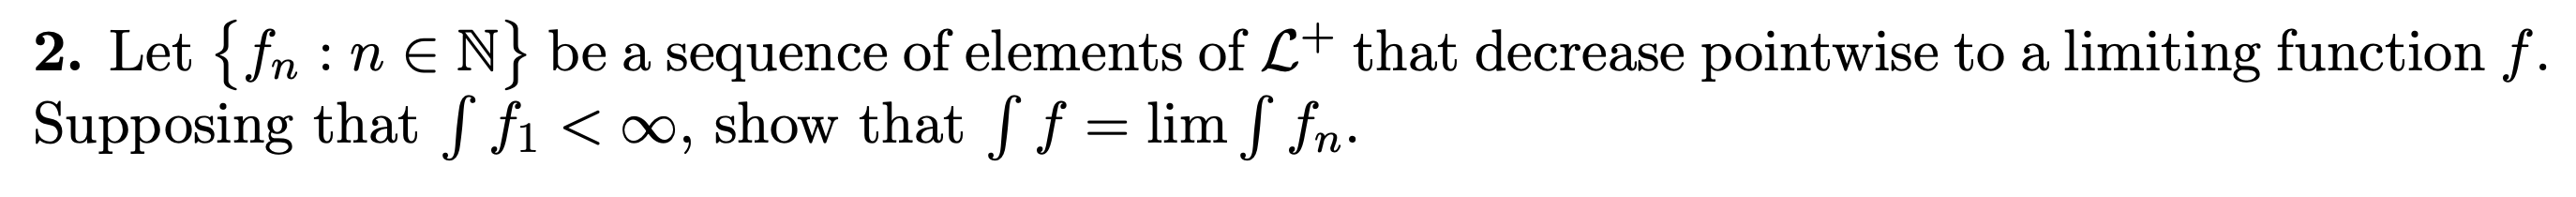
\includegraphics[width=400pt]{img/analysis--berkeley-202a-hw07-afc1.png}
\end{mdframed}

\begin{proof}
  Let $Z = \{x ~:~ f_1(x) = \infty\}$.

  Note that $\int f_1 < \infty$ implies $\mu(Z) = 0$. This follows from the fact
  that $\int_Z f_1 = \int \infty \cdot \ind_Z = \infty \cdot \mu(Z)$.

  Therefore
  \begin{align*}
    \int_X f &= \int_{X \setminus Z} f + \int_{Z} f \\
           &= \int_{X \setminus Z} f.
  \end{align*}
  Let $c = \sup \{f_1(x) ~:~ x \in X \setminus Z \}$ and note that $c < \infty$.

  Then $\((c - f_n)|_{X \setminus Z}\)$ is a non-negative sequence of measurable functions increasing
  to $(c - f)|_{X \setminus Z}$.

  Therefore $\int_{X \setminus Z} (c - f) = \lim_{n\to\infty} \int_{X \setminus Z} c - f_n$, by the monotone
  convergence theorem.

  Subtracting $c$ from both sides, and then multiplying both sides by $-1$, we
  obtain $\int_{X \setminus Z} f = \lim_{n\to\infty} \int_{X \setminus Z} f_n$.

  Thus we have shown that $\int f = \int_{X \setminus Z} f_n$.

  But $\mu(Z) = 0$, therefore $\int_{X \setminus Z} f_n = \int_{X} f_n - \int_{Z} f_n = \int_{X} f_n$.

  Therefore $\int_X f = \int_X f_n$ as required.
\end{proof}

\newpage
\begin{mdframed}
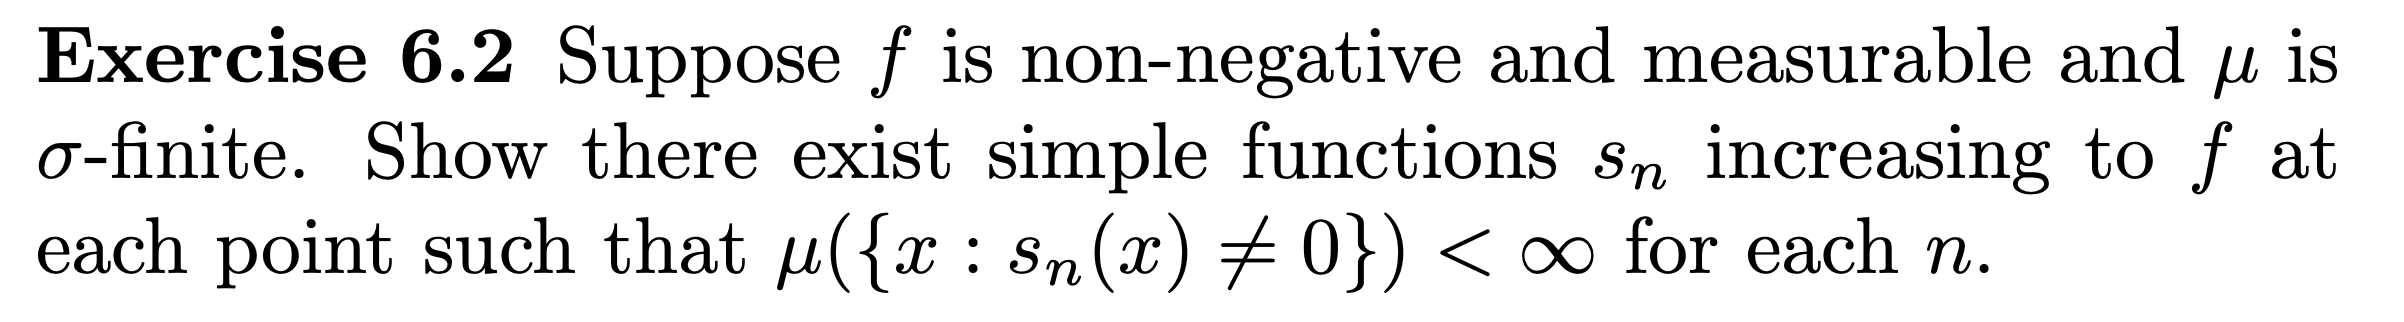
\includegraphics[width=400pt]{img/analysis--berkeley-202a-hw07-263d.png}
\end{mdframed}

\begin{proof}
  We first recall the standard construction (Bass proposition 5.14) of a sequence of non-negative simple
  functions increasing to $f$. For $n = 1, 2, \ldots$ and $i = 1, 2, \ldots, n2^n$, we define
  \begin{align*}
    A_{in} := \{x ~:~ \frac{i - 1}{2^n} < f(x) \leq \frac{i}{2^n} \}
  \end{align*}
  and
  \begin{align*}
    B_n := \{x ~:~ f(x) \geq n\}.
  \end{align*}
  Using these we define
  \begin{align*}
    s^*_n := n\ind_{B_n} + \sum_{i=1}^{n2^n} \frac{i-1}{2^n}\ind_{A_in}.
  \end{align*}
  We now modify this construction to yield $s_n$ satisfying the requirement
  that $\mu(\{x ~:~ s_n(x) > 0\}) < \infty$.

  Let $X$ be the set upon which $\mu$ is defined. Since $\mu$ is $\sigma$-finite we may choose a countable
  collection of pairwise disjoint sets $X_1, X_2, \ldots$ such that $\mu(X_i) < \infty$ for each $i$
  and $\bigcup_{i=1}^\infty = X$.

  We then define
  \begin{align*}
    s_n := s^*_n \ind_{\bigcup_{i=1}^n X_i}.
  \end{align*}
  To see that $s_n$ increases to $f$ at each point note that for every $x$ there exists $N \in \N$ such
  that $x \in {\bigcup_{i=1}^n X_i}$ for all $n > N$. Therefore the sequence $(s_n(x))_{n > N}$ is a tail of
  the sequence $s^*_n(x)$, which we know increases to $f(x)$ (Bass proposition 5.14).

  Finally we need to show that $\mu(\{x ~:~ s_n(x) > 0\}) < \infty$ for all $n$. For our construction, it
  suffices to show that $\mu\(\bigcup_{i=1}^n X_i\) < \infty$ for all $n$. This follows from countable
  additivity of $\mu$, since the $X_i$ are disjoint and each has finite measure.

  % Scott McIntyre
  % I'll construct a counterexample using an X that isn't sigma-finite. Let R* denote the measure space of real
  % numbers under the counting measure (the measure of a set is just the cardinality of that set, where infinite
  % sets give ∞). Define f: R* -> R by f(x) = 1 for all x. Take a sequence of simple functions s_n = ∑a_{i,n}
  % χ_{A_{i,n}} that increase to f; we can generate a new sequence of simple functions that increase to f by
  % setting all of the a_{i,n} to be 1 so that each s_n = ∑χ_{A_{i,n}}, where we force each of the A_{i,n} to be
  % disjoint for a given n. This also means we can rewrite that s_n as a characteristic function χ_{A_n}, so we
  % can find a sequence of characteristic functions increasing to f corresponding to any s_n increasing to f.
  % Suppose s_n satisfies the premise of (6.2). That means for the corresponding χ_{A_n}, each A_n can only be of
  % finite measure, and by our counting definition of measure, each A_n must be finite. This means the union of
  % all A_n is countable, so take any x not in any of the A_n. The limit of s_n(x) is just 0, but f(x) = 1, which
  % is a contradiction. Thus, such an s_n satisfying (6.2) cannot exist.

  % Dan
  % Let me just state my proposed solution: we take the standard construction of an increasing sequence of simple functions (Bass prop 5.14) and multiply it by the characteristic function of (-n, n). Questions:
  % Do you see something wrong with my solution?
  % In your counter-example, what formal claim are you proving? For example, are you proving this claim? "For a
  % non-sigma-finite measure there does not exist a sequence of simple functions s_n increasing to f such that
  % \mu({x: s_n(x) > 0}) < infty"
  % In my solution, I think that sigma-finiteness is necessary, but not sufficient. It is necessary because I
  % require that the measure space X can be covered by a monotone sequence of sets each of finite measure, and
  % this condition is equivalent to sigma-finiteness. But that does not show that my particular choice of
  % monotone sets do actually have finite measure for all sigma finite measures.

  % Scott McIntyre
  % 1. Your solution is only considering functions mapping from R to R, where you need a solution mapping from
  % any sigma finite X to R. However, your solution does indeed prove the claim for function mapping from R to R,
  % so try generalizing it.

  % 2. My counterexample is proving the claim that there exists functions such that no increasing sequence of
  % simple functions that are nonzero on a finite measure set can converge to that function. However, the problem
  % is saying that if you force the input space to be sigma finite, then any non-negative measurable will have a
  % sequence of simple functions all nonzero on a finite measure set that converges to that function.

  % 3. You found a solution that works for functions mapping R to R. Using intervals of the form [0,n] will
  % monotonically increase, but they won’t cover all of R. You don’t need any collection of monotone sets to be
  % sufficient; you just need to find a collection of monotone sets in in your input space X
\end{proof}

\newpage
\begin{mdframed}
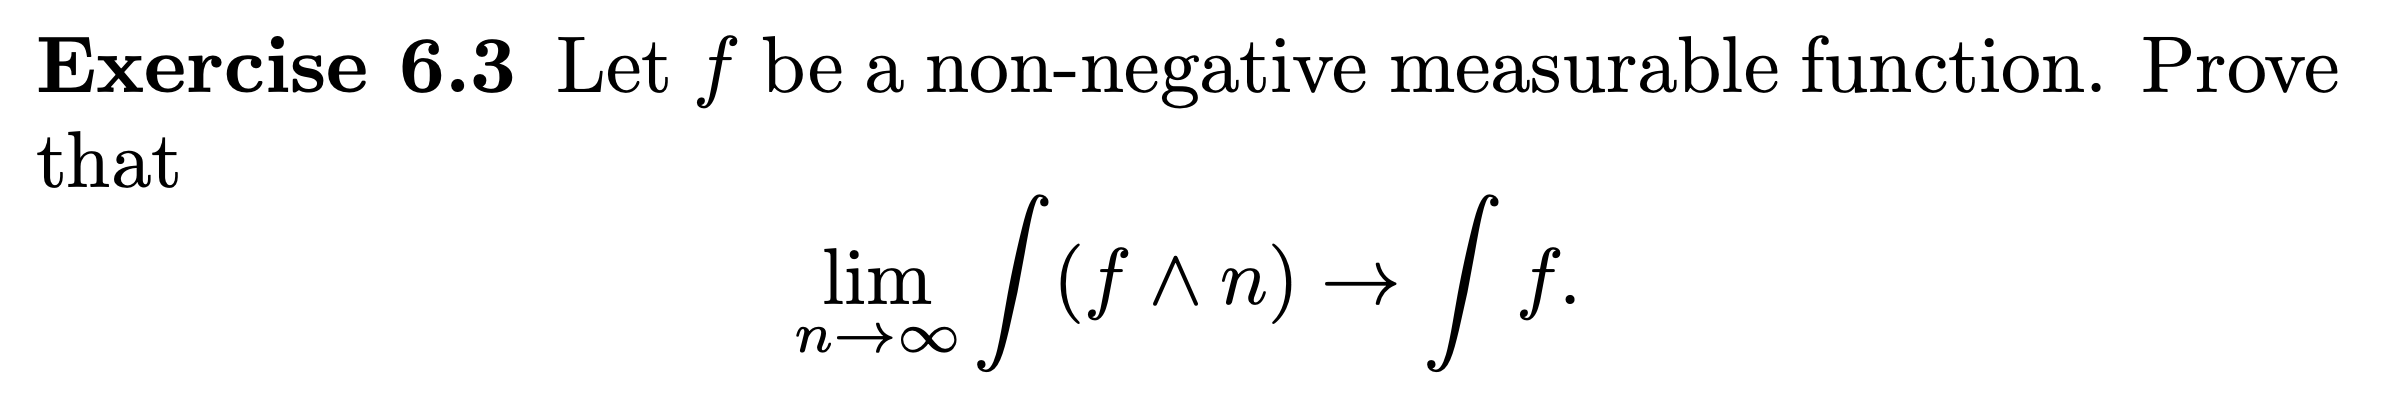
\includegraphics[width=400pt]{img/analysis--berkeley-202a-hw07-5290.png}
\end{mdframed}

\begin{proof}

  First suppose $f$ is finite. Let $N = \ceil{\sup f}$. Then $\int (f \land n) = \int f$ for all $n \geq N$.

  Let $H = \{x ~:~ f(x) = \infty\}$.

  First suppose $\mu(H) = 0$. Then
  \begin{align*}
    \lim_{n\to\infty} \int (f \land n) = \lim_{n\to\infty} \int_{H^c} (f \land n).
  \end{align*}
  Let $N = \ceil{\sup_{x \in H^c} f}$. Then $\int_{H^c} (f \land n) = \int_{H^c} f = \int f$ for
  all $n \geq N$.

  Therefore $\lim_{n\to\infty} \int (f \land n) = \int f$ as required.

  Next note that $\int_H (f \land n) = \int_H f$ for all $n$ and suppose that $\mu(H) > 0$.

  Therefore for all $n$ we
  have $\int (f \land n) \geq \int_H (f \land n) = \int_H f = \infty \cdot \mu(H) = \infty$, and
  therefore $\lim_{n\to\infty} \int (f \land n) = \infty$.

  But also $\int f \geq \infty \cdot \mu(H) = \infty$.

  Therefore again $\lim_{n\to\infty} \int (f \land n) = \int f$ as required.
\end{proof}

\newpage
\begin{mdframed}
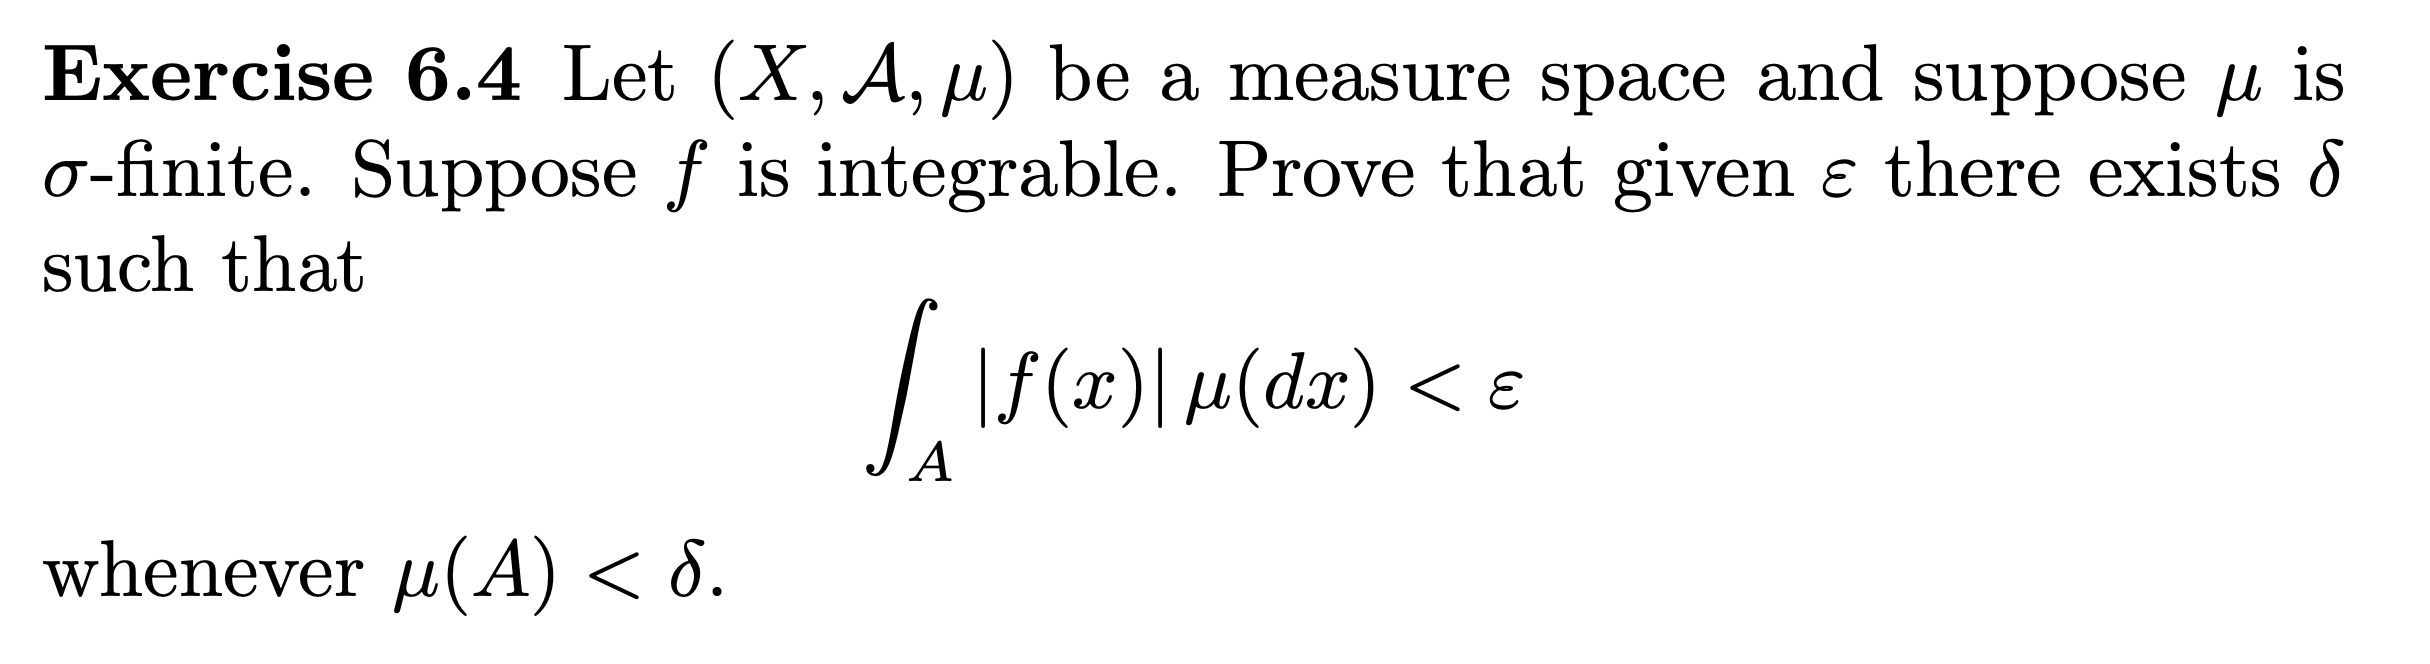
\includegraphics[width=400pt]{img/analysis--berkeley-202a-hw07-610e.png}
\end{mdframed}

% https://github.com/brennier/math-problems/blob/master/Class%20Problems/Real%20Analysis%20I/Problem%20Set%208.pdf
\begin{proof}
  Let $\eps > 0$.

  Since $|f|\ind_A \leq |f|$ we have $\int |f|\ind_A \leq \int |f| < \infty$. Therefore $|f|\ind_A$ is
  integrable, and therefore there exists a simple function $0 \leq s \leq |f|\ind_A$ a.e. such
  that $\int |f|\ind_A - \int s < \frac{\eps}{2}$.



\end{proof}

\begin{lemma}\label{lemma-integrable-fn-is-infinite-on-a-null-set}
  Suppose $f$ is integrable and let $I = \{x \in X ~:~ |f(x)| = \infty \}$. Then $\mu(I) = 0$.
\end{lemma}

\begin{proof}
  Note that
  \begin{align*}
    \int f &= \int_I f + \int_{X \setminus I} f \\
           &= \int_I f^+ - \int_I f^- + \int_{X \setminus I} f^+ - \int_{X \setminus I} f^-,
  \end{align*}
  where $f^+ = \max(f, 0)$ and $f^- = \max(-f, 0)$.

  Let $P = \{x \in X ~:~ f(x) > 0 \}$. Then
  \begin{align*}
    \int_I f^+ = \int_{I \cap P} f = \infty \cdot \mu(I \cap P),
  \end{align*}
  and
  \begin{align*}
    \int_I f^- = \int_{I \cap P^c} -f = \infty \cdot \mu(I \cap P^c).
  \end{align*}
  Suppose for a contradiction that $\mu(I) > 0$. Then either $\mu(I \cap P) > 0$ or $\mu(I \cap P^c) > 0$.
  Therefore either $\int_I f^+ = \infty$ or $\int_I f^- = \infty$. Therefore either $\int f$ does not exist
  or $\int |f| = \infty$. But $f$ is integrable, therefore $\mu(I) = 0$.
\end{proof}

\begin{claim*}
  For all $\eps > 0$ there exists $\delta > 0$ such that if $\mu(A) < \delta$ then $\int_A |f| < \eps$.
\end{claim*}

\begin{proof}
  Let $I = \{x \in X ~:~ |f(x)| = \infty \}$ and note that we have $\mu(I) = 0$ by lemma
  \eqref{lemma-integrable-fn-is-infinite-on-a-null-set}.

  Let $c = \sup \{|f(x)| ~:~ x \in A \setminus I\}$. Then
  \begin{align*}
    \int_A |f| &= \int_{A\setminus I} |f| \\
               &\leq c\mu(A \setminus I) \\
               &= c\mu(A).
  \end{align*}
  Set $\delta = \eps/2c$. Then $\mu(A) < \delta$ implies $\int_A |f| \leq \eps/2 < \eps$ as required.
\end{proof}

\newpage
\begin{mdframed}
  Suppose $\mu(X) < \infty$ and $f_n$ is a sequence of uniformly bounded real-valued measurable functions that
  converge pointwise to $f$. Prove that
\begin{align*}
  \lim_{n \to \infty} \Bigg( \int f_n \d\mu \Bigg) = \int f \d\mu.
\end{align*}
  This is sometimes called the {\it bounded convergence theorem}.
\end{mdframed}


\begin{proof}
  Since the $f_n$ are uniformly bounded, there exists $M \in \R$ such that $|f_n| < M$ for all $n$.

  Let $g_n = f_n + M$ for all $n$. Then $g_n$ is a non-negative sequence of functions that converges
  pointwise to $f + M$.

  Let $h_n(x) = \inf_{m \geq n} g_m(x)$ for all $x$ and for all $n$. Note that $h_n$ is an increasing sequence
  of non-negative functions, and furthermore that
  \begin{align*}
    \lim_{n \to \infty} h_n(x) =: \liminf_{n \to \infty} g_n(x) = \lim_{n \to \infty} g_n(x) = f(x) + M.
  \end{align*}
  Therefore $h_n$ is an increasing sequence of non-negative functions that converges pointwise to $f + M$. By
  the monotone convergence theorem we have
  \begin{mdframed}
    \begin{align*}
    \lim_{n\to\infty} \int (f_n + M) \d\mu = \int (f + M) \d\mu,
    \end{align*}
  \red{TODO} When I first wrote this proof I wrote the line above. But it now seems to me that all we have is
  \begin{align*}
    \lim_{n\to\infty} \int \inf_{m \geq n} g_m \d\mu = \int (f + M) \d\mu,
  \end{align*}
  \end{mdframed}
  and by linearity of the integral we have
  \begin{align*}
    \lim_{n\to\infty} \int f_n \d\mu + M \mu(X) = \int f \d\mu + M \mu(X).
  \end{align*}
  Since $\mu(X) < \infty$ we have
  \begin{align*}
    \lim_{n\to\infty} \int f_n \d\mu = \int f \d\mu,
  \end{align*}
  as required.
\end{proof}
